%
\documentclass[12pt]{ociamthesis}
\usepackage{tikz}
\newcommand{\id}{\mathrm{id}}
\begin{document}

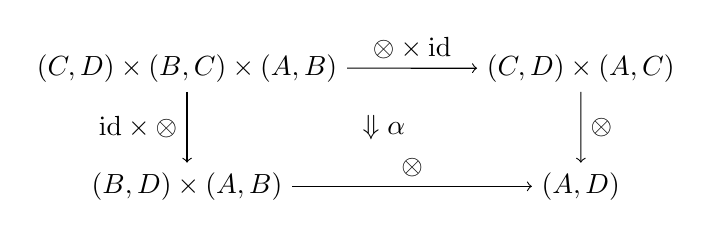
\begin{tikzpicture}[yscale=1.5, xscale=2.5]
\node (A) at (0,1){$\fB(C,D) \times \fB(B, C) \times \fB(A,B)$};
\node (C) at (2,1){$\fB(C,D) \times \fB(A,C)$};
\node (D) at (0,0) {$\fB(B,D)  \times \fB(A,B)$};
\node (E) at (2,0) {$\fB(A, D) $};
\node (B) at (1,.5) {$\Downarrow \alpha$};
\draw[->] (A) to node[above]{$\otimes \times \id$} (C);
\draw[->] (A) to node[left]{$\id \times \otimes$} (D);
\draw[->] (C) to node[right]{$\otimes$} (E);
\draw[->] (D) to node[above]{$\otimes$} (E);
\end{tikzpicture}
\end{document} 
